%
% $RCSfile$
%
% Copyright (c) 2005-2006. Christian Heller. All rights reserved.
%
% Permission is granted to copy, distribute and/or modify this document
% under the terms of the GNU Free Documentation License, Version 1.1 or
% any later version published by the Free Software Foundation; with no
% Invariant Sections, with no Front-Cover Texts and with no Back-Cover
% Texts. A copy of the license is included in the section entitled
% "GNU Free Documentation License".
%
% http://www.cybop.net
% - Cybernetics Oriented Programming -
%
% http://www.resmedicinae.org
% - Information in Medicine -
%
% Version: $Revision$ $Date$ $Author$
% Authors: Christian Heller <christian.heller@tuxtax.de>
%

\section{Reflexions on Concepts}
\label{reflexions_on_concepts_heading}

Although many of the ideas and solutions presented here, in a \emph{bottom-up}
manner, stem from writing source code in practice (following the
\emph{Constructive Development} method of research as announced in section
\ref{method_heading}), the overall approach and explanation of results follow a
\emph{top-down} path. High-level concepts are considered first, before moving
on to an implementation and proof in practice. Because of the steady comparison
to principles of nature and other sciences, this approach is called
\emph{cybernetics-oriented}, as explained in section \ref{idea_heading}. Figure
\ref{approach_figure} shows in which order the elements of CYBOP will be
considered.

\begin{figure}[ht]
    \begin{center}
        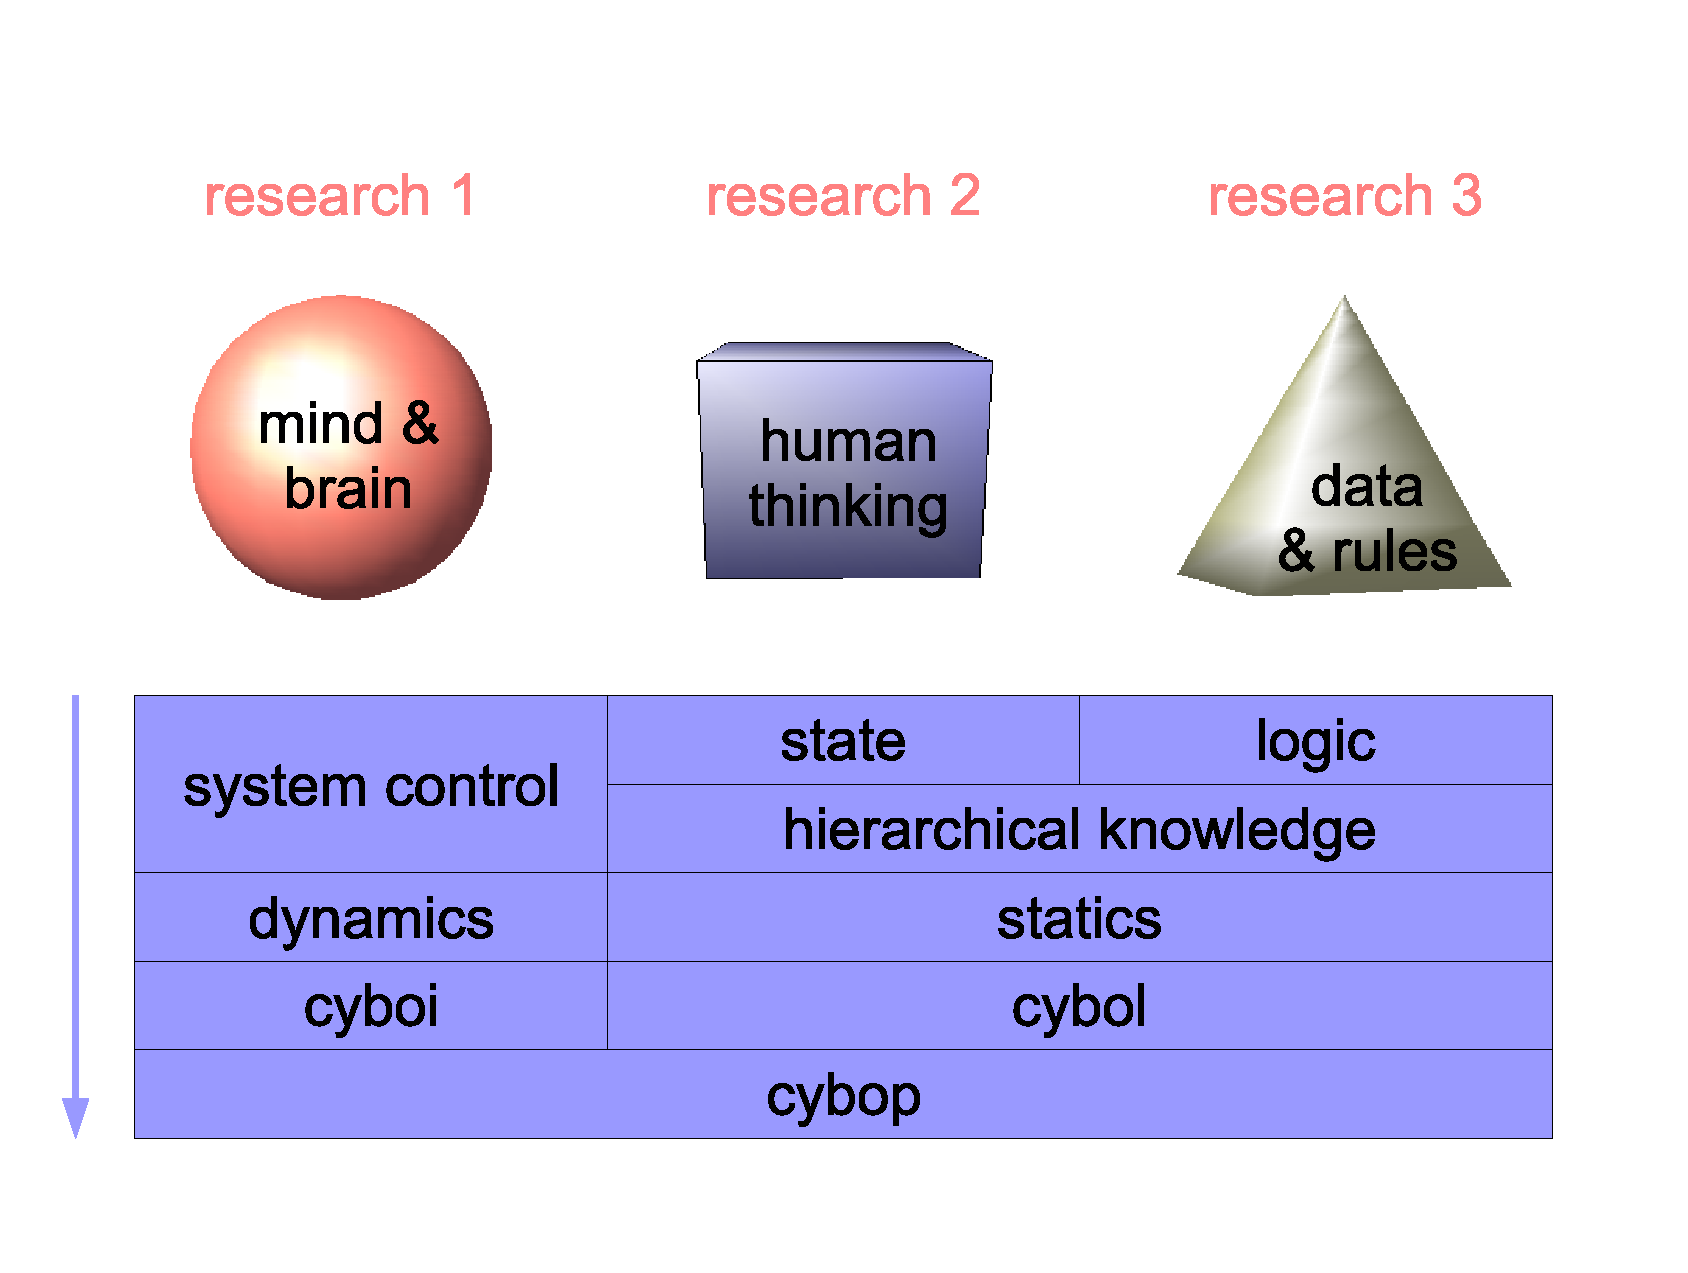
\includegraphics[scale=0.2]{vector/approach.eps}
        \caption{Consideration of CYBOP}
        \label{approach_figure}
    \end{center}
\end{figure}

A first observation, when looking at human beings from a philosophical
perspective, is the separation of \emph{Mind} and \emph{Brain} (Body).
Accordingly, CYBOP treats computers as \emph{Systems} owning and processing
\emph{Knowledge}. This is not unlike the idea of \emph{Agent} systems owning a
\emph{Knowledge Base} \cite{parks,kuehnel}. All abstract knowledge that humans
make up belongs to their mind. The brain is merely a physical carrier of
knowledge. Similarly, there are actually two kinds of software: one
representing \emph{passive} knowledge and the other \emph{actively} controlling
a system's hardware.

Secondly, attention is payed to the concepts of \emph{Human Thinking}
\cite{heller2004}, as investigated by psychology. Through their application,
knowledge becomes \emph{hierarchical}. Moreover, this work tried to embed
knowledge models in an environment of \emph{Dimensions}, as known from physics.
Every model keeps a number of \emph{Meta Information} about its parts.
\emph{Positions} in space or time are one such example.

Thirdly, \emph{State-} gets distinguished from \emph{Logic} knowledge. It is
known from neurological research that the human brain has special communication
regions that, simply spoken, do nothing else than translating data, i.e. an
input- into an output \emph{State}, according to rules of \emph{Logic}. Systems
theory uses similar abstractions. When talking about states, this work means a
composed \emph{Set} of states.

In CYBOP (figure \ref{approach_figure}), all knowledge (states and logic),
belongs to a system's \emph{Statics}, and is described by CYBOL language
templates (section \ref{cybol_heading}). The processing of knowledge at
runtime, to control a system, is \emph{Dynamics} and happens in the CYBOI
interpreter (section \ref{cyboi_heading}).

%
% $RCSfile: statics_and_dynamics.tex,v $
%
% Copyright (c) 2005-2006. Christian Heller. All rights reserved.
%
% Permission is granted to copy, distribute and/or modify this document
% under the terms of the GNU Free Documentation License, Version 1.1 or
% any later version published by the Free Software Foundation; with no
% Invariant Sections, with no Front-Cover Texts and with no Back-Cover
% Texts. A copy of the license is included in the section entitled
% "GNU Free Documentation License".
%
% http://www.cybop.net
% - Cybernetics Oriented Programming -
%
% http://www.resmedicinae.org
% - Information in Medicine -
%
% Version: $Revision: 1.1 $ $Date: 2006-01-03 08:21:45 $ $Author: christian $
% Authors: Christian Heller <christian.heller@tuxtax.de>
%

\subsection{Statics and Dynamics}
\label{statics_and_dynamics_heading}

Over the years, it has turned out to be helpful in software design, to separate
\emph{Domain Knowledge} from \emph{Application Functionality}. In
one-or-another form, the architectural\\software patterns \cite{heller2005}
\emph{Layers}, \emph{Domain Model} and \emph{Model View Controller} (MVC) all
suggest to apply this principle.

The \emph{Tools \& Materials} approach \cite{tandm}\\talks of \emph{active}
applications (tools) working on \emph{passive} domain data (material). And also
\emph{System Family Engineering} (section \ref{architectural_troubles_heading})
bases on a separate treatment of domain and application, in form of
\emph{Domain Engineering} (DE) and \emph{Application Engineering} (AE).

An often neglected fact of these approaches is that not only the domain, but
also the application contains important business knowledge (figure
\ref{separation_figure}). The \emph{User Interface} (UI), for example, is
tailored for a specific business domain. And the logic behind, if not
contained in the UI itself, is often put in a \emph{Controller} which belongs
to the application$-$, not the domain layer.

\begin{figure}[ht]
    \begin{center}
        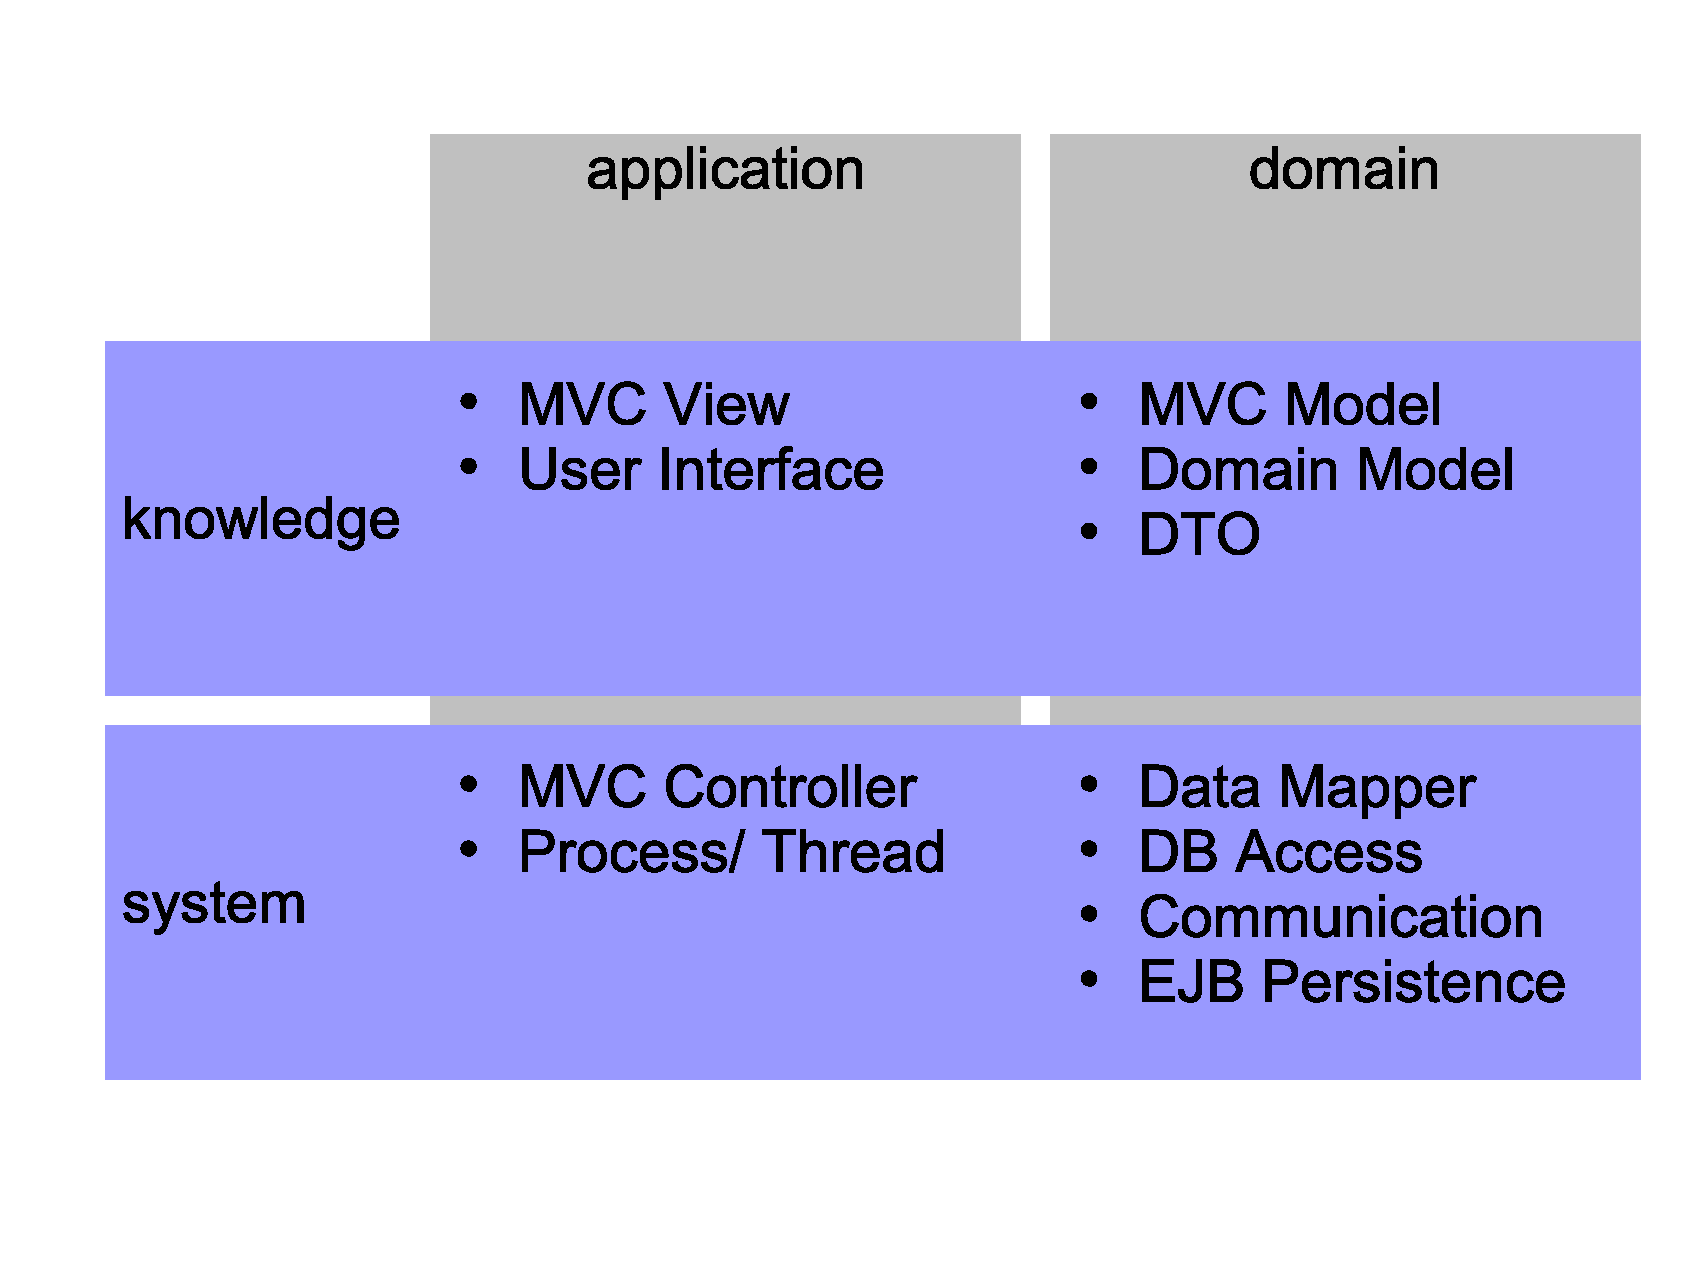
\includegraphics[scale=0.2]{vector/separation.eps}
        \caption{Different Knowledge Separations}
        \label{separation_figure}
    \end{center}
\end{figure}

Similarly, the domain often contains functionality which actually does belong
into the application process: \emph{Database} (DB) access is handled by help of
patterns like the \emph{Data Mapper} \cite{heller2005}, in which the mapper\\
objects contain \emph{Structured Query Language} (SQL) code to connect to a
\emph{Database Management System} (DBMS); \emph{Enterprise Java Beans} (EJB),
which should better be pure domain objects, imitate a \emph{Middleware}
providing persistence- or communication mechanisms, which originally have
nothing to do with the business knowledge they contain.

It is precisely this \emph{Mixup} of responsibilities between an application
system and its domain knowledge, that leads to multiple inter-dependencies and
hence unflexibility within a system. Instead, a separation should be made
between active \emph{System Control} and passive \emph{Knowledge}. A UI's
appearance would then be treated as domain knowledge, just as the logic of the
functions called through it. A data mapper would be transformed into a simple
\emph{Translator} -- similar to a \emph{Data Transfer Object} (DTO)
\cite{heller2005} -- that knows how to convert data from one domain model into
another; its DBMS access functionality, however, would be extracted and put
into the application system. Monstrosities like EJBs would likewise be opened
up and parted into their actual domain knowledge, and all other mechanisms
around -- the latter being moved into the application system.

To sum up this thought: The essential realisation here is that hardware-close
mechanisms like the ones necessary for data input/ output (i/o), enabling
inter-system communication, should be handled in an active application system
layer which was started as process on a computer, and \emph{not} be merged with
pure, passive domain knowledge. User interfaces and other data models which are
traditionally hold in the application layer, should rather belong to the domain
layer, together with all other business knowledge.

Now, if a distinction of high-level knowledge from low-level system control
software is considered to be useful, the next question must be: \textit{How,
that is in which form, best to store knowledge in a system?}

One possible structure called \emph{Data Garden} \cite{holland} was proposed by
Wau Holland of the \emph{Chaos Computer Club} (CCC). Although being a
non-academic organisation, his ideas on knowledge modelling are interesting to
this work. He dreamt of whole \emph{Forests}, \emph{Parks} or -- as the name
says -- \emph{Gardens} of \emph{Knowledge Trees} and \emph{Data Bushes} (figure
\ref{garden_figure}).

\begin{figure}[ht]
    \begin{center}
        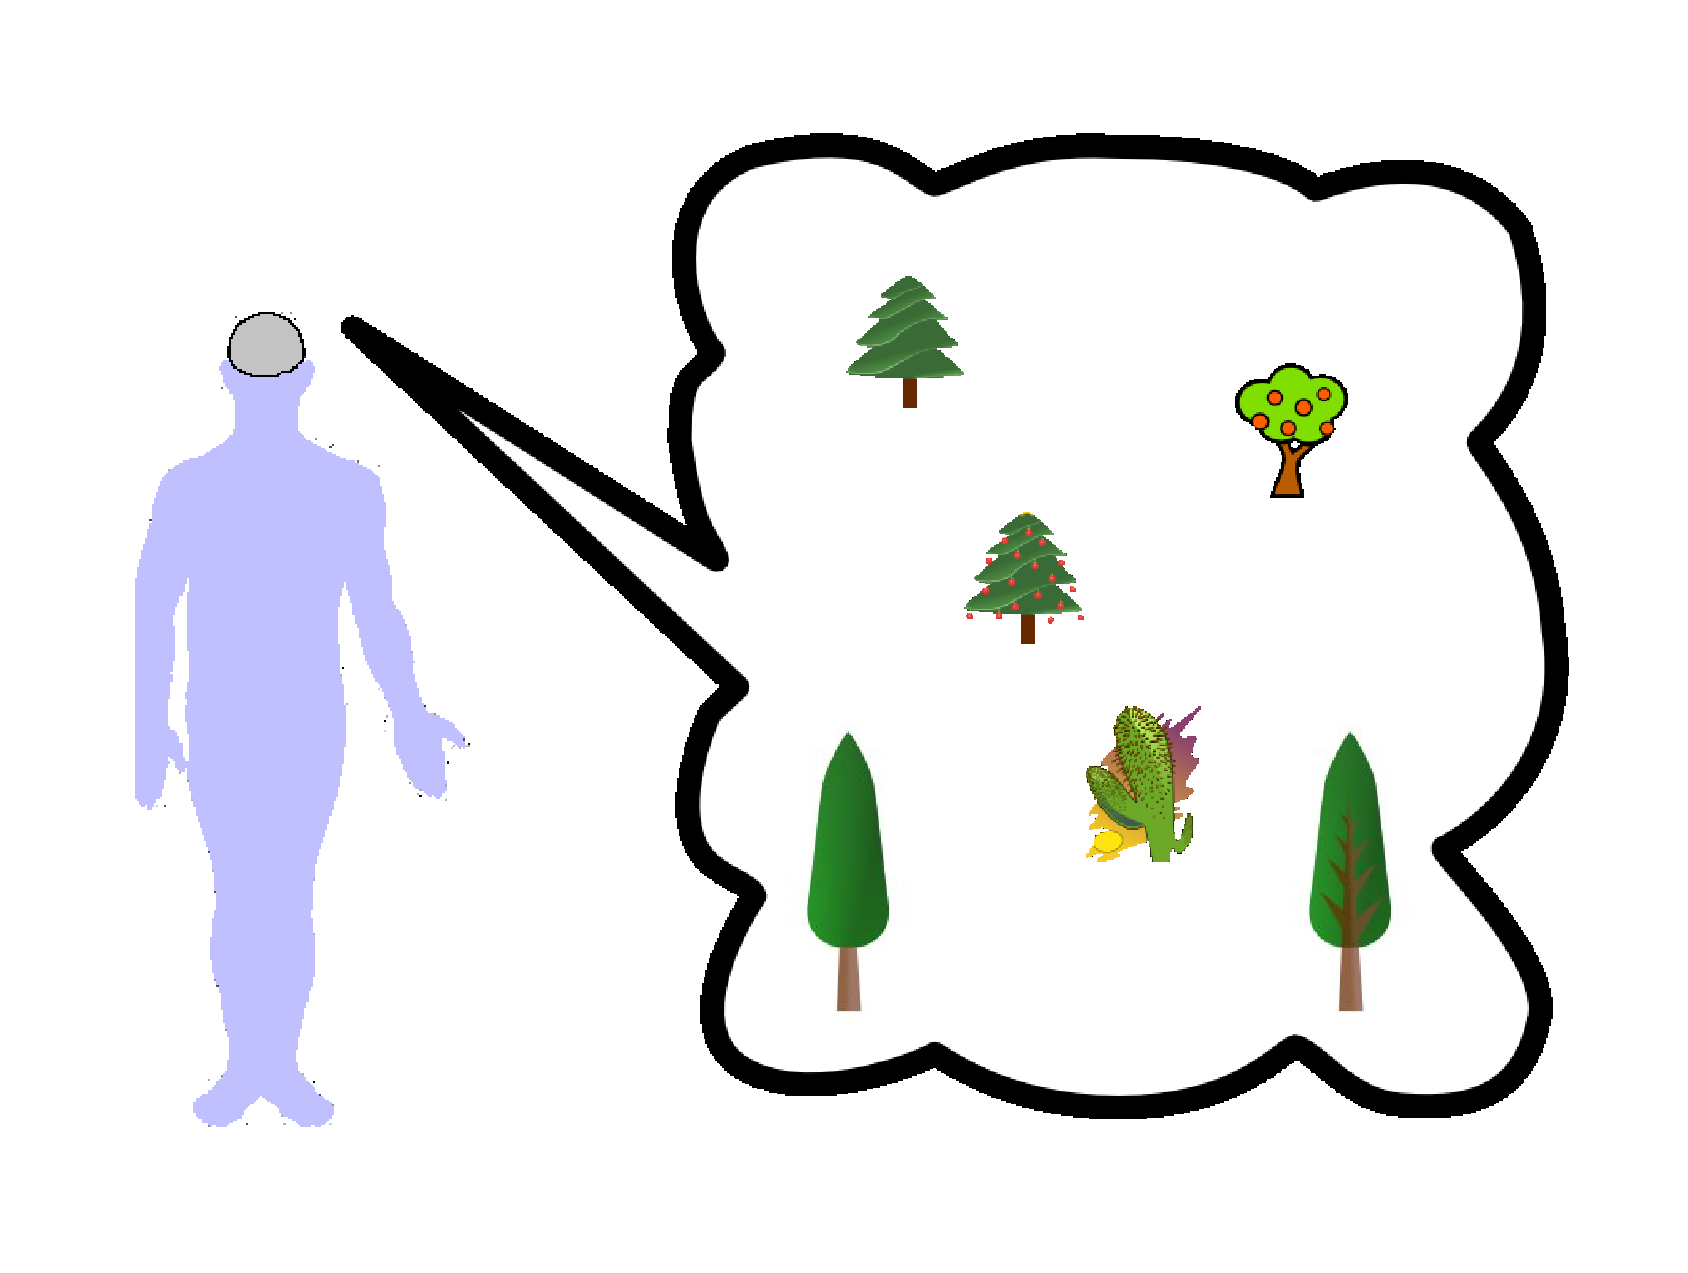
\includegraphics[scale=0.2]{vector/garden.eps}
        \caption{Data Garden}
        \label{garden_figure}
    \end{center}
\end{figure}

The interpreter created in the work described in this article stores all its
knowledge in \emph{one single} tree, whose root node it references. The single
concepts (data bushes) are represented by branches of that knowledge tree.

Further arguments in favour of a distinction of statics and dynamics are: mind
\& body (philosophy), cerebral cortex \& communication regions (neurology),
genetic information \& cell body (biology), long- \& short-term memory
(psychology), and more.

%
% $RCSfile: knowledge_schema.tex,v $
%
% Copyright (c) 2005-2006. Christian Heller. All rights reserved.
%
% Permission is granted to copy, distribute and/or modify this document
% under the terms of the GNU Free Documentation License, Version 1.1 or
% any later version published by the Free Software Foundation; with no
% Invariant Sections, with no Front-Cover Texts and with no Back-Cover
% Texts. A copy of the license is included in the section entitled
% "GNU Free Documentation License".
%
% http://www.cybop.net
% - Cybernetics Oriented Programming -
%
% http://www.resmedicinae.org
% - Information in Medicine -
%
% Version: $Revision: 1.1 $ $Date: 2006-01-03 08:21:45 $ $Author: christian $
% Authors: Christian Heller <christian.heller@tuxtax.de>
%

\subsection{Knowledge Schema}
\label{knowledge_schema_heading}

Human beings have a brain which they use to think, in other words to build up a
mind. While the former exists in the \emph{Real World}, the latter is
constructed as a subjective \emph{Virtual World}. All people do think, all the
time, even not knowing that they do. One would therefore guess that the act of
\emph{Thinking} is a most common one, familiar to anybody. But judging from the
enormous research effort in sciences dealing with it, the \emph{Principles}
behind thinking are not that easy to grasp.

%
% $RCSfile: schema.tex,v $
%
% Copyright (c) 2005-2006. Christian Heller. All rights reserved.
%
% Permission is granted to copy, distribute and/or modify this document
% under the terms of the GNU Free Documentation License, Version 1.1 or
% any later version published by the Free Software Foundation; with no
% Invariant Sections, with no Front-Cover Texts and with no Back-Cover
% Texts. A copy of the license is included in the section entitled
% "GNU Free Documentation License".
%
% http://www.cybop.net
% - Cybernetics Oriented Programming -
%
% http://www.resmedicinae.org
% - Information in Medicine -
%
% Version: $Revision: 1.1 $ $Date: 2006-01-03 08:21:45 $ $Author: christian $
% Authors: Christian Heller <christian.heller@tuxtax.de>
%

\subsubsection{Schema}
\label{schema_heading}

A theoretical \emph{Model} is an abstract clip of the real world, and exists in
the human mind. Another common word for \emph{Model} is \emph{Concept}. It is
the subsumption of \emph{Item}, \emph{Category} and \emph{Compound}, resulting
from three activities of abstraction: \emph{Discrimination},
\emph{Categorisation} and \emph{Composition} \cite{heller2004}. Each model
\emph{knows} about the parts it consists of.

\begin{figure}[ht]
    \begin{center}
        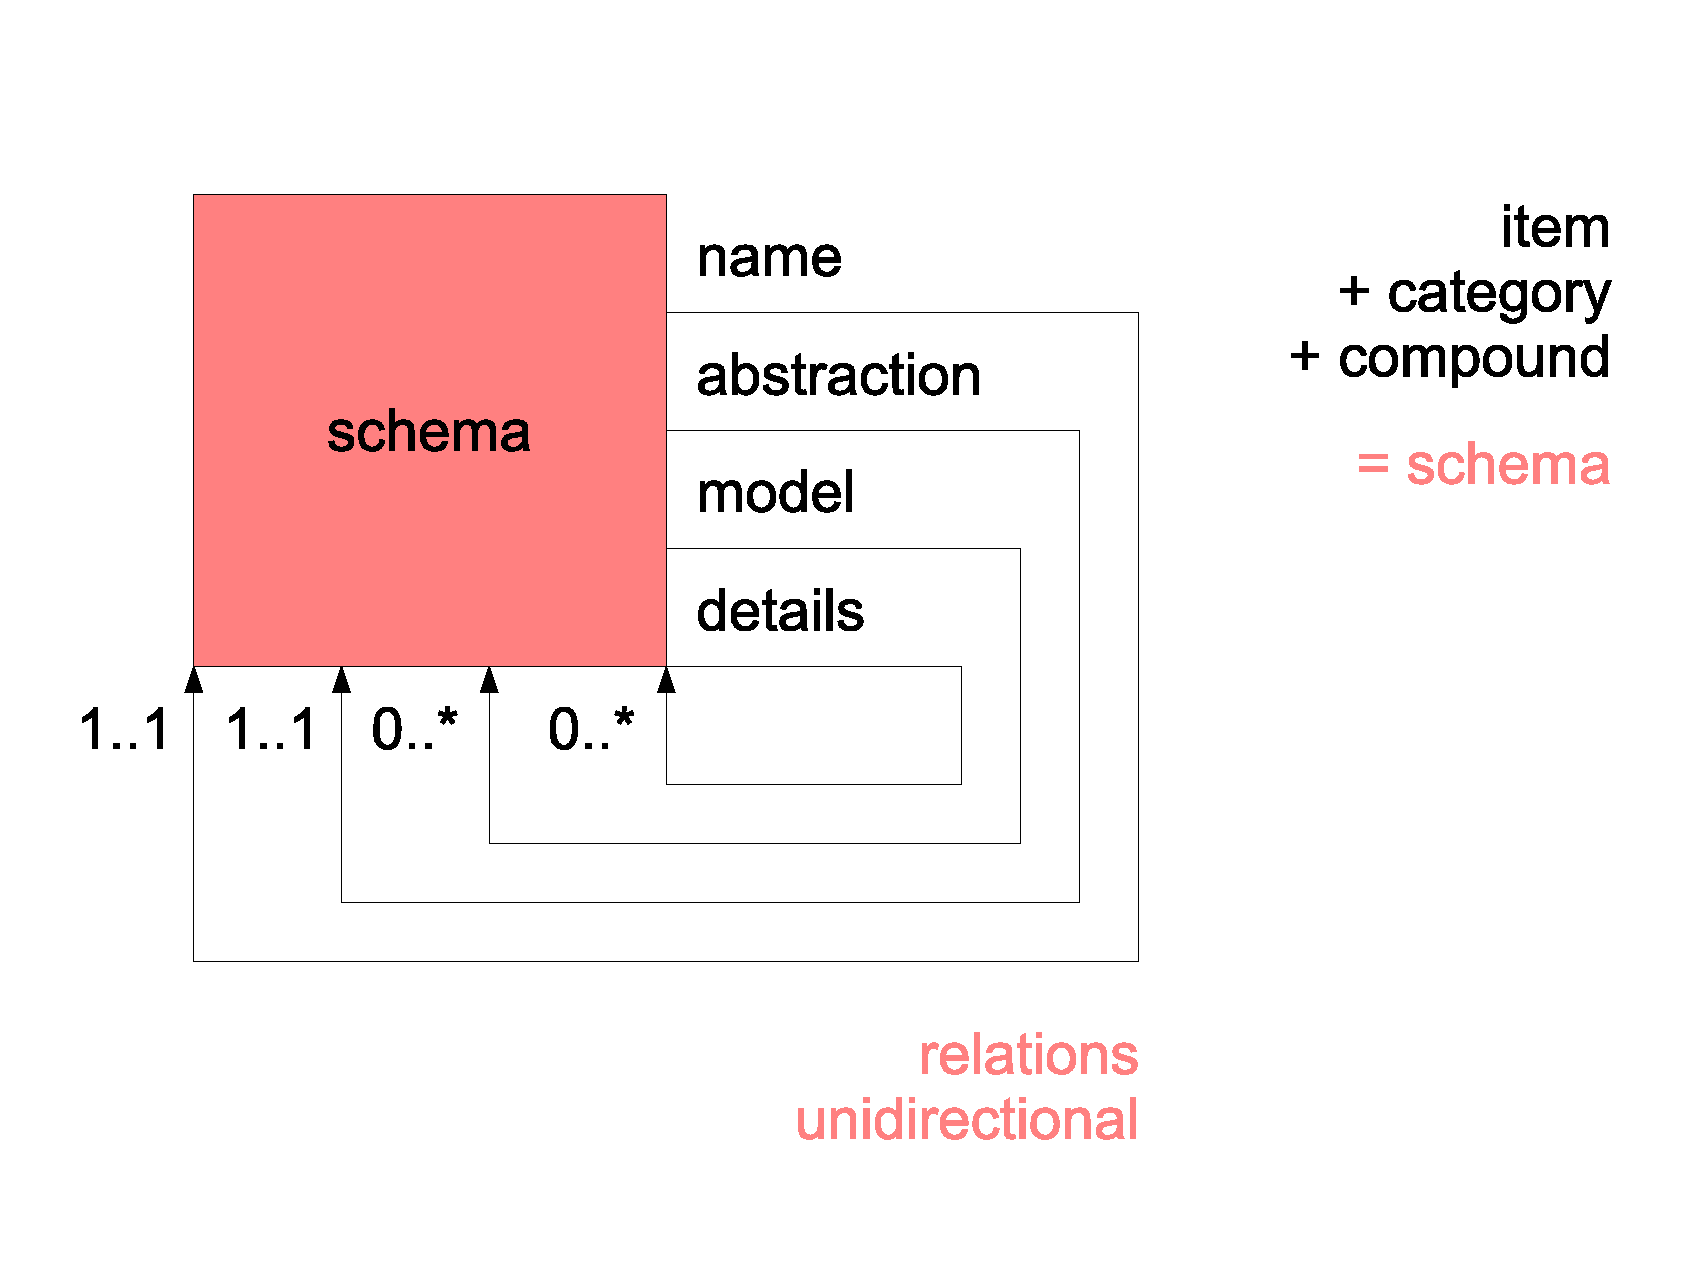
\includegraphics[scale=0.2]{vector/schema.eps}
        \caption{Knowledge Schema}
        \label{schema_figure}
    \end{center}
\end{figure}

Yet what does this knowledge of a compound model (whole) about its parts imply?
Software developers call knowledge \emph{about} something
\emph{Meta Information}. Figure \ref{schema_figure} illustrates a
\emph{Schema} (structure) with four kinds of meta information in a whole-part
relation.

An obvious way is to give each part a unique \emph{Name} for identification.
Secondly, a compound needs to know about the \emph{Model} of each part since a
part may itself be seen as compound that needs to know about its parts. The
distinction of the several kinds of models, in other words the kind of
\emph{Abstraction} (compound, term, number etc.) of a model is the third kind
of information a compound needs to know about its parts. It is comparable to a
\emph{Type} in classical system programming languages. All further kinds of
meta information are summed up by a fourth relation which is called
\emph{Details}.

%
% $RCSfile: double_hierarchy.tex,v $
%
% Copyright (C) 2002-2008. Christian Heller.
%
% Permission is granted to copy, distribute and/or modify this document
% under the terms of the GNU Free Documentation License, Version 1.1 or
% any later version published by the Free Software Foundation; with no
% Invariant Sections, with no Front-Cover Texts and with no Back-Cover
% Texts. A copy of the license is included in the section entitled
% "GNU Free Documentation License".
%
% http://www.cybop.net
% - Cybernetics Oriented Programming -
%
% http://www.resmedicinae.org
% - Information in Medicine -
%
% Version: $Revision: 1.1 $ $Date: 2008-08-19 20:41:06 $ $Author: christian $
% Authors: Christian Heller <christian.heller@tuxtax.de>
%

\subsection{Double Hierarchy}
\label{double_hierarchy_heading}
\index{Double Hierarchy}
\index{Whole-Part Relationship}
\index{Dialectical Relationship between Whole and Part}
\index{Conceptual Interaction}
\index{Part}
\index{Property}
\index{Constraint}

Finally, what makes up the character of a model (in the understanding of the
human mind) is a combination of two hierarchies: the \emph{Parts} it consists
of, together with \emph{Meta Information} about it.

Most properties of a molecule in \emph{Chemistry}, for example, are determined
by the number and arrangement of its atoms. \emph{Hydrogen} (H$_{2}$) becomes
\emph{Water} (H$_{2}$O) (with a totally different character) when just one
\emph{Oxygen} (O) atom is added per hydrogen molecule. The Wikipedia Encyclopedia
\cite{wikipedia} cites and writes about Richard Levins and Richard Lewontin
who, in their book \textit{The Dialectical Biologist} \cite{levins}, sketch a
\emph{dialectical} approach to biology:

\begin{quote}
    They focus on the (dialectical) relationship between the \emph{Whole} (or
    \emph{Totality}) and the \emph{Parts}: \textit{Part makes Whole, and Whole
    makes Part} \cite[p. 272]{levins}. That is, a biological system of some kind
    consists of a collection of heterogeneous parts. All of these contribute to
    the character of the whole, as in reductionist thinking. On the other hand,
    the whole has an existence independent of the parts and feeds back to affect
    and determine the nature of the parts. This back-and-forth (dialectic) of
    causation implies a dynamic process. \ldots\ Further, each species is part
    of the \emph{Environment} of all of the others.
\end{quote}

The kinds of meta information discussed in the previous sections were also
called \emph{Dimensions} or \emph{Conceptual Interaction} between a \emph{Whole}
and its \emph{Parts}. They may represent very different properties and each of
them may be constrained to certain values- or areas of validity.

\begin{figure}[ht]
    \begin{center}
        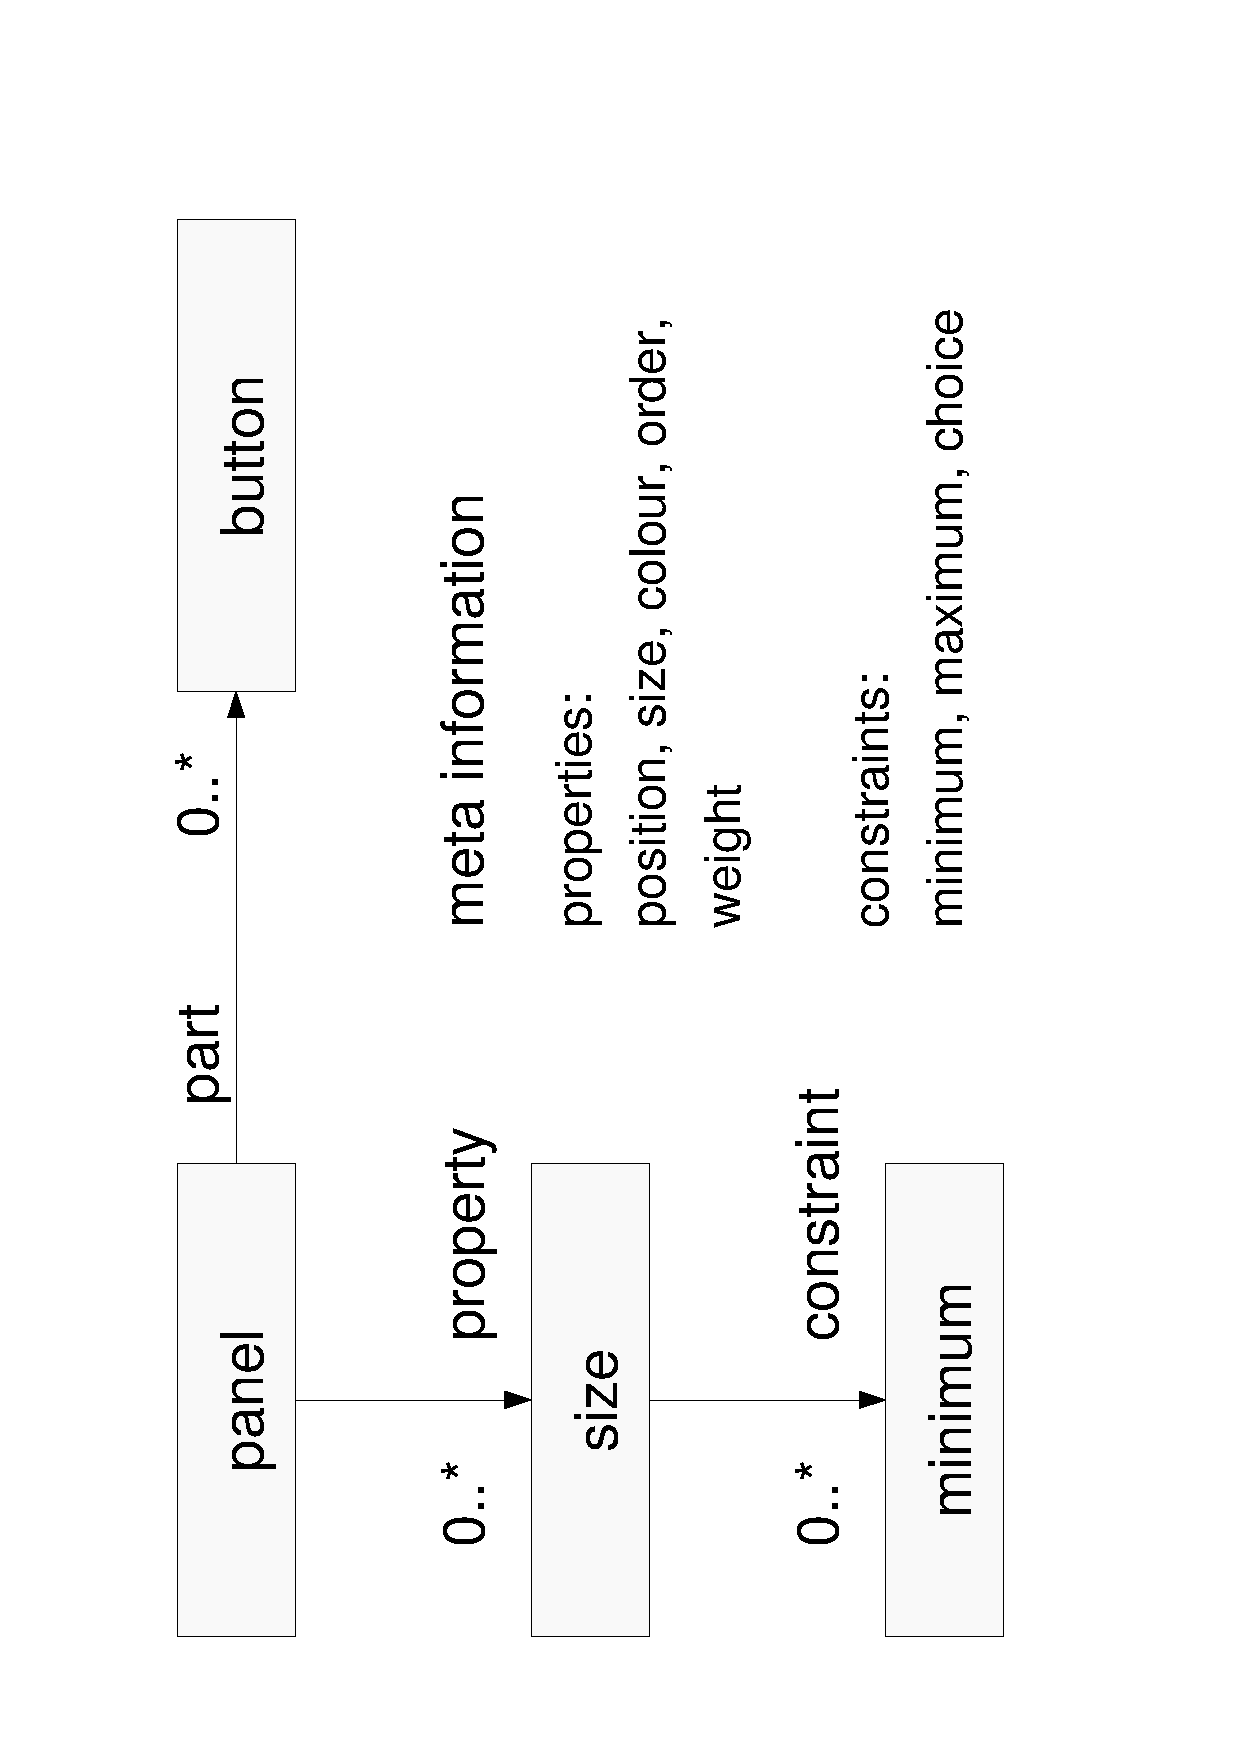
\includegraphics[scale=0.3,angle=-90]{graphic/double.pdf}
        \caption{Double Hierarchy of Parts and Meta Information}
        \label{double_figure}
    \end{center}
\end{figure}

Figure \ref{double_figure} illustrates the \emph{Double Hierarchy} here
spoken of. A graphical panel was chosen as example model. It may consist of
smaller parts, among them being a number of buttons. Altogether, they form the
\emph{Part Hierarchy}. On the other hand, there are properties like the size,
position or colour of the buttons, which are neither part of the panel, nor of
the buttons themselves; they are information \emph{about} the buttons and form
an own \emph{Meta Hierarchy}. To the latter do also belong constraints like the
minimum size of a button or a possible choice of colours for it. Constraints can
be treated like meta information about properties. Once again: \emph{Properties}
are information about a \emph{Part}; \emph{Constraints} are information about a
\emph{Property}.


%
% $RCSfile: state_and_logic.tex,v $
%
% Copyright (c) 2005-2006. Christian Heller. All rights reserved.
%
% Permission is granted to copy, distribute and/or modify this document
% under the terms of the GNU Free Documentation License, Version 1.1 or
% any later version published by the Free Software Foundation; with no
% Invariant Sections, with no Front-Cover Texts and with no Back-Cover
% Texts. A copy of the license is included in the section entitled
% "GNU Free Documentation License".
%
% http://www.cybop.net
% - Cybernetics Oriented Programming -
%
% http://www.resmedicinae.org
% - Information in Medicine -
%
% Version: $Revision: 1.1 $ $Date: 2006-01-03 08:21:45 $ $Author: christian $
% Authors: Christian Heller <christian.heller@tuxtax.de>
%

\subsection{State and Logic}
\label{state_and_logic_heading}

According to the observations made in the work described in this article, there
are two kinds of knowledge: \emph{State-} and \emph{Logic}. While the former
may be placed in a spatial dimension, the latter is processed as sequence over
time. Often, logic is labelled \emph{dynamic} behaviour -- but only the
\emph{execution} of a rule of logic is dynamic, \emph{not} the rule itself
(\emph{static}).

Rules of logic translate input- into output states. What
characterises a system is how it applies logic knowledge to translate state
knowledge \cite{heller2002}. Yet how to imagine a knowledge model consisting of
state- as well as logic parts? Following an example.

The famous \emph{Model View Controller} (MVC) pattern was extended by the
\emph{Hierarchical MVC} (HMVC) pattern towards a hierarchy of \emph{MVC Triads}
\cite{cai}. The omnipresence of hierarchies in the MVC was demonstrated in
\cite{hellerbohl}.

\begin{figure}[ht]
    \begin{center}
        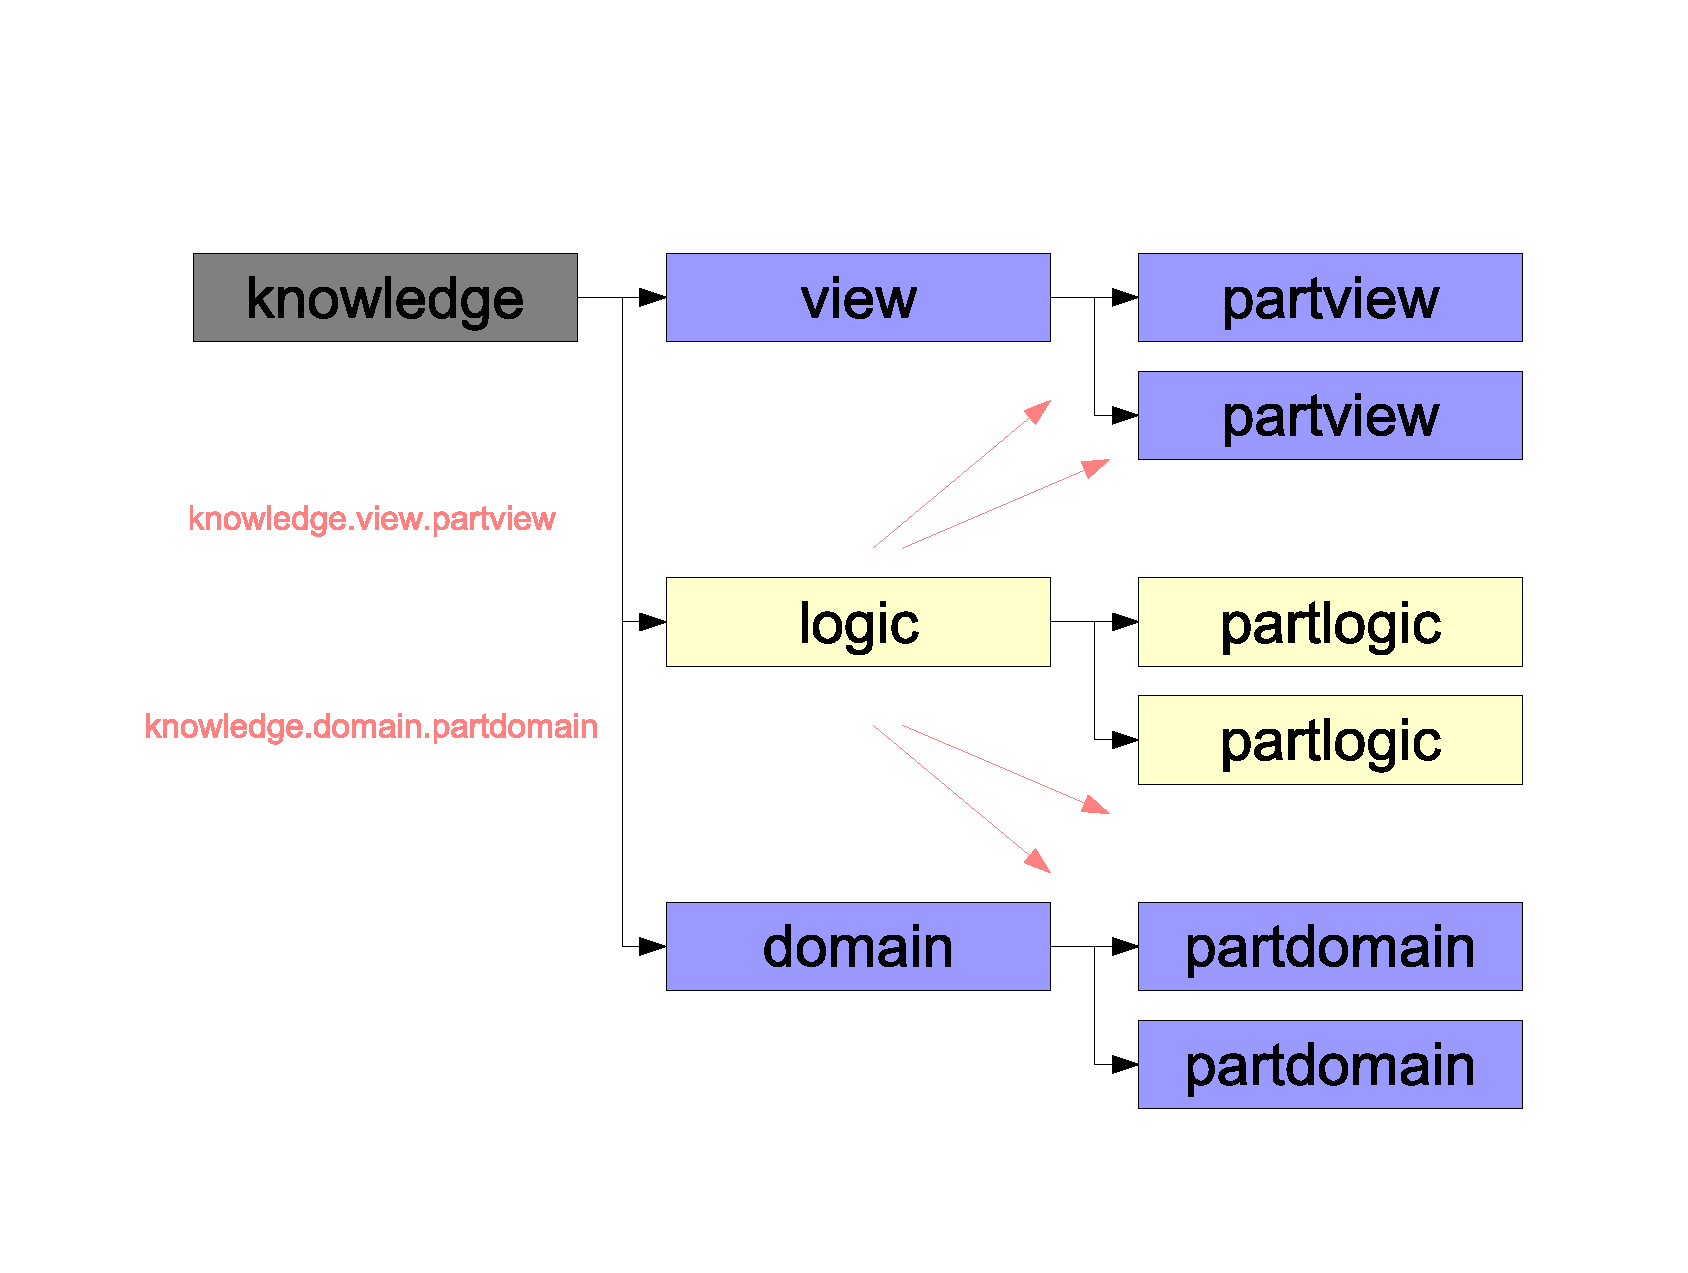
\includegraphics[scale=0.2]{vector/mvctree.eps}
        \caption{Runtime Logic manipulating States}
        \label{mvctree_figure}
    \end{center}
\end{figure}

Figure \ref{mvctree_figure} shows the three parts: \emph{Domain} (Model),
\emph{View} and \emph{Logic} (Controller) of an (adapted) MVC pattern as
independent branches of one common knowledge tree, as existent at system
runtime in memory. Each of them represents a concept on its own. The logic
model, however, is allowed to access and change the view- and domain model; it
is able to link different knowledge models. But view- and domain model,
representing states, are not allowed to manipulate logic. In other words: The
dependencies between logic- and state models are \emph{unidirectional}.

An innovation is that logic knowledge gets manipulatable. A logic model
(algorithm) cannot only access and change state-, but also logic models, even
itself! Because models modified in that manner can be made persistent in form
of CYBOL knowledge templates (section \ref{practical_proof_heading}), and be
reloaded the next time an application starts, this may be seen as a kind of
\emph{Meta Programming} \cite{wikipedia}.

The clear separation of states and logic into discrete models avoids unwanted
dependencies as caused by the bundling of attributes and methods in OOP. All
that would be needed to make a CYBOP system work with new state models, is the
corresponding translation logic. Translators \cite{hellerkunze} simplify
architectures and unify communication.

